% =====================================================================
% SOICT 2026 — bản tiếng Việt chi tiết (để tập nói và để đọc)
% Bài báo: papers/soict2026/manuscript/main.tex
% Bản trình bày chính thức (tiếng Anh, ~7:30): ../soict2026/main.tex
% Biên dịch: ./compile.sh   (XeLaTeX; bản kèm ghi chú: NOTES=1 ./compile.sh)
%
% Nguyên tắc: mỗi slide một thông điệp, lời thường trên slide, thuật ngữ trong
% ngoặc, chi tiết ở ghi chú và slide dự phòng. Số liệu lấy từ bài báo, riêng
% slide về cổng lọc lấy từ results/ml_08_anomaly_gate/gate_operating_points.csv
% và jetson/model/anomaly_threshold.json.
%
% KẾ HOẠCH THỜI GIAN (~11:00). Nếu chỉ có 7 phút: bỏ các slide "Vì sao bộ
% phân loại là Random Forest", "Kết quả 2" và "Kết quả 3", chỉ nói câu kết luận của chúng.
% Sau slide tài liệu tham khảo là DỰ PHÒNG cho hỏi đáp.
% =====================================================================
\documentclass[aspectratio=169, 11pt]{beamer}
% =====================================================================
% Shared Beamer preamble for all decks in slides/
%   - 16:9, metropolis theme, Okabe-Ito colorblind-safe accents
%   - XeLaTeX + fontspec with a Vietnamese-capable sans fallback chain
%   - Speaker notes: compile with \def\shownotes{} to get the notes PDF
% Input this file right after \documentclass in each deck.
% =====================================================================

\usetheme{metropolis}
\metroset{block=fill, numbering=fraction, progressbar=frametitle, sectionpage=progressbar}

\usepackage{fontspec}
\usepackage{graphicx}
\usepackage{booktabs}
\usepackage{multirow}
\usepackage{amsmath,amssymb}
\usepackage{xcolor}
\usepackage{tikz}
\usetikzlibrary{positioning, arrows.meta, shapes.geometric, fit, backgrounds, calc}
\usepackage{appendixnumberbeamer}

% ---------------------------------------------------------------------
% Fonts. TeX Gyre Heros is the portable first choice (ships with a full
% TeX Live and covers Vietnamese); on a BasicTeX/macOS box it is absent,
% so fall back to system sans fonts that still carry Vietnamese
% diacritics, and only as a last resort to the serif TeX Gyre Termes
% (which is always present) rather than silently hitting nullfont.
% ---------------------------------------------------------------------
\IfFontExistsTF{TeX Gyre Heros}
  {\setsansfont{TeX Gyre Heros}[Ligatures=TeX]}
  {\IfFontExistsTF{Helvetica Neue}
     {\setsansfont{Helvetica Neue}[Ligatures=TeX]}
     {\IfFontExistsTF{Arial}
        {\setsansfont{Arial}[Ligatures=TeX]}
        {\setsansfont{TeX Gyre Termes}[Ligatures=TeX]}}}
\IfFontExistsTF{Menlo}
  {\setmonofont{Menlo}[Scale=0.82]}
  {\IfFontExistsTF{TeX Gyre Cursor}{\setmonofont{TeX Gyre Cursor}[Scale=0.85]}{}}

% ---------------------------------------------------------------------
% Palette. Blue and green follow the Okabe-Ito accents used in the
% manuscript TikZ figures; the emphasis accent is a red rather than
% Okabe-Ito's vermillion, so highlighted numbers read unambiguously as
% "look here" from the back of the room.
% ---------------------------------------------------------------------
\definecolor{accBlue}{HTML}{0072B2}
\definecolor{accGreen}{HTML}{009E73}
\definecolor{accRed}{HTML}{C1121F}
\definecolor{inkDark}{HTML}{23373B}

\setbeamercolor{frametitle}{bg=accBlue, fg=white}
\setbeamercolor{progress bar}{fg=accRed, bg=accRed!25}
\setbeamercolor{progress bar in head/foot}{fg=accRed, bg=accBlue!25}
\setbeamercolor{progress bar in section page}{fg=accRed, bg=accRed!25}
\setbeamercolor{alerted text}{fg=accRed}
\setbeamercolor{example text}{fg=accGreen}
\setbeamercolor{block title}{bg=accBlue!12, fg=inkDark}
\setbeamercolor{block body}{bg=accBlue!5}
\setbeamercolor{block title alerted}{bg=accRed!15, fg=inkDark}
\setbeamercolor{block body alerted}{bg=accRed!6}
\setbeamercolor{block title example}{bg=accGreen!15, fg=inkDark}
\setbeamercolor{block body example}{bg=accGreen!6}

% [standout] frames: metropolis paints them dark teal. Use the same blue as
% the frame titles so the closing slide reads as part of the same deck, and
% size the text up — it is meant to be seen from the back of the room.
\setbeamercolor{palette primary}{bg=accBlue, fg=white}
\setbeamerfont{standout}{size=\huge, series=\bfseries}

% Metropolis draws no bullet glyph by default; a small square reads better
% from the back of a conference room than pure indentation.
\setbeamertemplate{itemize item}{\raisebox{0.12ex}{\tiny$\blacksquare$}}
\setbeamertemplate{itemize subitem}{\raisebox{0.12ex}{\tiny$\square$}}
\setbeamercolor{itemize item}{fg=accBlue}
\setbeamercolor{itemize subitem}{fg=accBlue!70}

% Vietnamese has few hyphenation points, so a long run of words can fail to
% break and stick out past the text block. Allow looser interword glue as a
% last resort instead of an overfull line.
\setlength{\emergencystretch}{2em}

% Tables: booktabs rules look thin on a projector.
\setlength{\heavyrulewidth}{1.1pt}
\setlength{\lightrulewidth}{0.6pt}
\renewcommand{\arraystretch}{1.15}

% ---------------------------------------------------------------------
% Centre the title page and the section pages. Metropolis left-aligns both
% (\raggedright inside its templates); all three decks here want them
% centred, so each calls \centeredtitles right after loading this file.
% It stays a macro rather than an unconditional override so a future deck
% can keep the stock metropolis alignment by simply not calling it.
% ---------------------------------------------------------------------
\makeatletter
\newcommand{\centeredtitles}{%
  % Applied through \AtBeginDocument: metropolis re-applies its own inner
  % templates at \begin{document}, so overrides installed earlier are
  % silently reverted.
  \AtBeginDocument{%
    % Metropolis' title page puts the title graphic in a \vbox to 0pt at the
    % very top of a bottom-aligned \paperheight minipage — the image loads but
    % lands off the top of the page. Rebuild the title page with the graphic
    % after the opening \vfill, where it is actually visible.
    \setbeamertemplate{title graphic}{}%
    \setbeamertemplate{title page}{%
      \begin{minipage}[b][\paperheight]{\textwidth}
        \vfill
        \centering
        \ifx\inserttitlegraphic\@empty\else
          \inserttitlegraphic\par\vspace*{1.1em}%
        \fi
        \ifx\inserttitle\@empty\else\usebeamertemplate*{title}\fi
        \ifx\insertsubtitle\@empty\else\usebeamertemplate*{subtitle}\fi
        \usebeamertemplate*{title separator}
        \ifx\beamer@shortauthor\@empty\else\usebeamertemplate*{author}\fi
        \ifx\insertdate\@empty\else\usebeamertemplate*{date}\fi
        \ifx\insertinstitute\@empty\else\usebeamertemplate*{institute}\fi
        \vfill
        \vspace*{1mm}
      \end{minipage}}%
    \setbeamertemplate{title}{%
      \centering\linespread{1.0}\inserttitle\par\vspace*{0.5em}}%
    \setbeamertemplate{subtitle}{%
      \centering\insertsubtitle\par\vspace*{0.5em}}%
    \setbeamertemplate{author}{%
      \vspace*{2em}\centering\insertauthor\par\vspace*{0.25em}}%
    \setbeamertemplate{date}{%
      \centering\insertdate\par}%
    \setbeamertemplate{institute}{%
      \vspace*{3mm}\centering\insertinstitute\par}%
    % Same as metropolis' "progressbar" section page, but centred. No deck
    % here uses subsections, so that branch of the original is dropped.
    \setbeamertemplate{section page}{%
      \centering
      \begin{minipage}{22em}
        \centering
        \usebeamercolor[fg]{section title}%
        \usebeamerfont{section title}%
        \insertsectionhead\\[-1ex]
        \usebeamertemplate*{progress bar in section page}%
        \par
      \end{minipage}
      \par
      \vspace{\baselineskip}}%
  }%
}
\makeatother

% Shrink a box to the available width, but only when it would otherwise
% overflow. A tabular that is wider than its beamer column is NOT clipped —
% it silently overprints the neighbouring column — so every table that sits
% inside \begin{columns} goes through this.
\newcommand{\fitwidth}[1]{%
  \resizebox{\ifdim\width>\linewidth\linewidth\else\width\fi}{!}{#1}}

% ---------------------------------------------------------------------
% Emphasis macros used throughout the decks.
% ---------------------------------------------------------------------
\newcommand{\key}[1]{\textcolor{accBlue}{\textbf{#1}}}
\newcommand{\good}[1]{\textcolor{accGreen}{\textbf{#1}}}
\newcommand{\bad}[1]{\textcolor{accRed}{\textbf{#1}}}
\newcommand{\num}[1]{\textcolor{accRed}{\textbf{#1}}}

% One-line "so what" strip, pinned at the bottom of a result slide.
% Kept deliberately compact: this box sits directly above metropolis' frame
% number, so any extra height here pushes text into the footer and the page
% number ends up printed on top of the last line.
\newcommand{\takeaway}[1]{%
  \vfill
  \begin{beamercolorbox}[wd=\textwidth, sep=4pt, rounded=true]{block body example}%
    \footnotesize #1%
  \end{beamercolorbox}}

% ---------------------------------------------------------------------
% Speaker notes. Build the plain deck normally; build the notes version
% with:  xelatex "\def\shownotes{}% =====================================================================
% SOICT 2026 — bản tiếng Việt chi tiết (để tập nói và để đọc)
% Bài báo: papers/soict2026/manuscript/main.tex
% Bản trình bày chính thức (tiếng Anh, ~7:30): ../soict2026/main.tex
% Biên dịch: ./compile.sh   (XeLaTeX; bản kèm ghi chú: NOTES=1 ./compile.sh)
%
% Nguyên tắc: mỗi slide một thông điệp, lời thường trên slide, thuật ngữ trong
% ngoặc, chi tiết ở ghi chú và slide dự phòng. Số liệu lấy từ bài báo, riêng
% slide về cổng lọc lấy từ results/ml_08_anomaly_gate/gate_operating_points.csv
% và jetson/model/anomaly_threshold.json.
%
% KẾ HOẠCH THỜI GIAN (~11:00). Nếu chỉ có 7 phút: bỏ các slide "Vì sao bộ
% phân loại là Random Forest", "Kết quả 2" và "Kết quả 3", chỉ nói câu kết luận của chúng.
% Sau slide tài liệu tham khảo là DỰ PHÒNG cho hỏi đáp.
% =====================================================================
\documentclass[aspectratio=169, 11pt]{beamer}
% =====================================================================
% Shared Beamer preamble for all decks in slides/
%   - 16:9, metropolis theme, Okabe-Ito colorblind-safe accents
%   - XeLaTeX + fontspec with a Vietnamese-capable sans fallback chain
%   - Speaker notes: compile with \def\shownotes{} to get the notes PDF
% Input this file right after \documentclass in each deck.
% =====================================================================

\usetheme{metropolis}
\metroset{block=fill, numbering=fraction, progressbar=frametitle, sectionpage=progressbar}

\usepackage{fontspec}
\usepackage{graphicx}
\usepackage{booktabs}
\usepackage{multirow}
\usepackage{amsmath,amssymb}
\usepackage{xcolor}
\usepackage{tikz}
\usetikzlibrary{positioning, arrows.meta, shapes.geometric, fit, backgrounds, calc}
\usepackage{appendixnumberbeamer}

% ---------------------------------------------------------------------
% Fonts. TeX Gyre Heros is the portable first choice (ships with a full
% TeX Live and covers Vietnamese); on a BasicTeX/macOS box it is absent,
% so fall back to system sans fonts that still carry Vietnamese
% diacritics, and only as a last resort to the serif TeX Gyre Termes
% (which is always present) rather than silently hitting nullfont.
% ---------------------------------------------------------------------
\IfFontExistsTF{TeX Gyre Heros}
  {\setsansfont{TeX Gyre Heros}[Ligatures=TeX]}
  {\IfFontExistsTF{Helvetica Neue}
     {\setsansfont{Helvetica Neue}[Ligatures=TeX]}
     {\IfFontExistsTF{Arial}
        {\setsansfont{Arial}[Ligatures=TeX]}
        {\setsansfont{TeX Gyre Termes}[Ligatures=TeX]}}}
\IfFontExistsTF{Menlo}
  {\setmonofont{Menlo}[Scale=0.82]}
  {\IfFontExistsTF{TeX Gyre Cursor}{\setmonofont{TeX Gyre Cursor}[Scale=0.85]}{}}

% ---------------------------------------------------------------------
% Palette. Blue and green follow the Okabe-Ito accents used in the
% manuscript TikZ figures; the emphasis accent is a red rather than
% Okabe-Ito's vermillion, so highlighted numbers read unambiguously as
% "look here" from the back of the room.
% ---------------------------------------------------------------------
\definecolor{accBlue}{HTML}{0072B2}
\definecolor{accGreen}{HTML}{009E73}
\definecolor{accRed}{HTML}{C1121F}
\definecolor{inkDark}{HTML}{23373B}

\setbeamercolor{frametitle}{bg=accBlue, fg=white}
\setbeamercolor{progress bar}{fg=accRed, bg=accRed!25}
\setbeamercolor{progress bar in head/foot}{fg=accRed, bg=accBlue!25}
\setbeamercolor{progress bar in section page}{fg=accRed, bg=accRed!25}
\setbeamercolor{alerted text}{fg=accRed}
\setbeamercolor{example text}{fg=accGreen}
\setbeamercolor{block title}{bg=accBlue!12, fg=inkDark}
\setbeamercolor{block body}{bg=accBlue!5}
\setbeamercolor{block title alerted}{bg=accRed!15, fg=inkDark}
\setbeamercolor{block body alerted}{bg=accRed!6}
\setbeamercolor{block title example}{bg=accGreen!15, fg=inkDark}
\setbeamercolor{block body example}{bg=accGreen!6}

% [standout] frames: metropolis paints them dark teal. Use the same blue as
% the frame titles so the closing slide reads as part of the same deck, and
% size the text up — it is meant to be seen from the back of the room.
\setbeamercolor{palette primary}{bg=accBlue, fg=white}
\setbeamerfont{standout}{size=\huge, series=\bfseries}

% Metropolis draws no bullet glyph by default; a small square reads better
% from the back of a conference room than pure indentation.
\setbeamertemplate{itemize item}{\raisebox{0.12ex}{\tiny$\blacksquare$}}
\setbeamertemplate{itemize subitem}{\raisebox{0.12ex}{\tiny$\square$}}
\setbeamercolor{itemize item}{fg=accBlue}
\setbeamercolor{itemize subitem}{fg=accBlue!70}

% Vietnamese has few hyphenation points, so a long run of words can fail to
% break and stick out past the text block. Allow looser interword glue as a
% last resort instead of an overfull line.
\setlength{\emergencystretch}{2em}

% Tables: booktabs rules look thin on a projector.
\setlength{\heavyrulewidth}{1.1pt}
\setlength{\lightrulewidth}{0.6pt}
\renewcommand{\arraystretch}{1.15}

% ---------------------------------------------------------------------
% Centre the title page and the section pages. Metropolis left-aligns both
% (\raggedright inside its templates); all three decks here want them
% centred, so each calls \centeredtitles right after loading this file.
% It stays a macro rather than an unconditional override so a future deck
% can keep the stock metropolis alignment by simply not calling it.
% ---------------------------------------------------------------------
\makeatletter
\newcommand{\centeredtitles}{%
  % Applied through \AtBeginDocument: metropolis re-applies its own inner
  % templates at \begin{document}, so overrides installed earlier are
  % silently reverted.
  \AtBeginDocument{%
    % Metropolis' title page puts the title graphic in a \vbox to 0pt at the
    % very top of a bottom-aligned \paperheight minipage — the image loads but
    % lands off the top of the page. Rebuild the title page with the graphic
    % after the opening \vfill, where it is actually visible.
    \setbeamertemplate{title graphic}{}%
    \setbeamertemplate{title page}{%
      \begin{minipage}[b][\paperheight]{\textwidth}
        \vfill
        \centering
        \ifx\inserttitlegraphic\@empty\else
          \inserttitlegraphic\par\vspace*{1.1em}%
        \fi
        \ifx\inserttitle\@empty\else\usebeamertemplate*{title}\fi
        \ifx\insertsubtitle\@empty\else\usebeamertemplate*{subtitle}\fi
        \usebeamertemplate*{title separator}
        \ifx\beamer@shortauthor\@empty\else\usebeamertemplate*{author}\fi
        \ifx\insertdate\@empty\else\usebeamertemplate*{date}\fi
        \ifx\insertinstitute\@empty\else\usebeamertemplate*{institute}\fi
        \vfill
        \vspace*{1mm}
      \end{minipage}}%
    \setbeamertemplate{title}{%
      \centering\linespread{1.0}\inserttitle\par\vspace*{0.5em}}%
    \setbeamertemplate{subtitle}{%
      \centering\insertsubtitle\par\vspace*{0.5em}}%
    \setbeamertemplate{author}{%
      \vspace*{2em}\centering\insertauthor\par\vspace*{0.25em}}%
    \setbeamertemplate{date}{%
      \centering\insertdate\par}%
    \setbeamertemplate{institute}{%
      \vspace*{3mm}\centering\insertinstitute\par}%
    % Same as metropolis' "progressbar" section page, but centred. No deck
    % here uses subsections, so that branch of the original is dropped.
    \setbeamertemplate{section page}{%
      \centering
      \begin{minipage}{22em}
        \centering
        \usebeamercolor[fg]{section title}%
        \usebeamerfont{section title}%
        \insertsectionhead\\[-1ex]
        \usebeamertemplate*{progress bar in section page}%
        \par
      \end{minipage}
      \par
      \vspace{\baselineskip}}%
  }%
}
\makeatother

% Shrink a box to the available width, but only when it would otherwise
% overflow. A tabular that is wider than its beamer column is NOT clipped —
% it silently overprints the neighbouring column — so every table that sits
% inside \begin{columns} goes through this.
\newcommand{\fitwidth}[1]{%
  \resizebox{\ifdim\width>\linewidth\linewidth\else\width\fi}{!}{#1}}

% ---------------------------------------------------------------------
% Emphasis macros used throughout the decks.
% ---------------------------------------------------------------------
\newcommand{\key}[1]{\textcolor{accBlue}{\textbf{#1}}}
\newcommand{\good}[1]{\textcolor{accGreen}{\textbf{#1}}}
\newcommand{\bad}[1]{\textcolor{accRed}{\textbf{#1}}}
\newcommand{\num}[1]{\textcolor{accRed}{\textbf{#1}}}

% One-line "so what" strip, pinned at the bottom of a result slide.
% Kept deliberately compact: this box sits directly above metropolis' frame
% number, so any extra height here pushes text into the footer and the page
% number ends up printed on top of the last line.
\newcommand{\takeaway}[1]{%
  \vfill
  \begin{beamercolorbox}[wd=\textwidth, sep=4pt, rounded=true]{block body example}%
    \footnotesize #1%
  \end{beamercolorbox}}

% ---------------------------------------------------------------------
% Speaker notes. Build the plain deck normally; build the notes version
% with:  xelatex "\def\shownotes{}\input{main.tex}"
% ---------------------------------------------------------------------
\ifdefined\shownotes
  \usepackage{pgfpages}
  \setbeameroption{show notes on second screen=right}
\fi

\centeredtitles

\graphicspath{%
  {../../papers/soict2026/results/benchmarks/}%
  {../../papers/soict2026/figures/}%
  {../../results/ml_08_anomaly_gate/}%
  {../../results/ml_07_cross_method_comparison/}%
}

\title{Hệ thống phát hiện xâm nhập phân tán thời gian thực trên cụm thiết bị biên Jetson Orin Nano Super với Kafka và PySpark}
\author{\textbf{Nguyễn Vũ Thái}\inst{1} \and Bùi Văn Dũng\inst{2} \and Đỗ Trí Nhựt\inst{2} \and Nguyễn Văn Dũ\inst{3}}
\institute{\scriptsize
           \inst{1}Phân hiệu tại TP.\ Hồ Chí Minh, Trường Đại học Giao thông Vận tải, TP.\ Hồ Chí Minh, Việt Nam \\
           \inst{2}Trường Đại học Công nghệ Thông tin, ĐHQG-HCM, TP.\ Hồ Chí Minh, Việt Nam \\
           \inst{3}Khoa Công nghệ Thông tin, Trường Đại học Nông Lâm, TP.\ Hồ Chí Minh, Việt Nam}
\date{SOICT 2026}

\begin{document}

% ---------------------------------------------------------------- 0:20
\maketitle
\note{Câu hỏi của bài: có hai bo mạch biên thì nên chia việc phát hiện xâm nhập
giữa chúng thế nào, và bo thứ hai thực sự đem lại bao nhiêu.}

% =====================================================================
\section{I.\ VẤN ĐỀ VÀ ĐÓNG GÓP}
% =====================================================================

% ---------------------------------------------------------------- 0:45
\begin{frame}{Phát hiện xâm nhập ngay tại thiết bị biên: còn ba khoảng trống}
  \begin{columns}[T]
    \begin{column}{0.55\textwidth}
      Mô hình phát hiện xâm nhập nay đã \emph{chạy được} trên bo mạch nhỏ, nhưng
      nếu một bo phải xét \key{mọi} luồng thì nó quá tải rất nhanh.
      \vspace{0.6em}

      \textbf{Nghiên cứu trước còn thiếu}
      \begin{enumerate}
        \item Chỉ đo trên \bad{một thiết bị}, không chia việc cho nhiều bo.
        \item Hiếm khi báo \bad{cùng lúc} tốc độ, độ trễ và năng lượng.
        \item Điểm số offline lấy từ quy trình \bad{rò rỉ dữ liệu}.
      \end{enumerate}
    \end{column}
    \begin{column}{0.40\textwidth}
      \begin{alertblock}{Câu hỏi}
        Có hai bo Jetson thì nên \emph{đặt} việc phát hiện lên chúng thế nào?
      \end{alertblock}
      \begin{exampleblock}{Cách làm}
        Tách làm hai: \key{cổng lọc} rẻ trên bo \#1, \key{bộ phân loại}
        nặng trên bo \#2, nối bằng Kafka.
      \end{exampleblock}
    \end{column}
  \end{columns}
  \note{Khoảng trống thứ ba là lý do nhóm làm bài FAIR về quy trình đánh giá
  chống rò rỉ.}
\end{frame}

% ---------------------------------------------------------------- 0:30
\begin{frame}{Các đóng góp}
  \begin{enumerate}
    \setlength{\itemsep}{0.4em}
    \item Hệ thống phát hiện xâm nhập \key{hai tầng, phân tán}: cổng lọc và
          bộ phân loại Spark đặt trên hai bo khác nhau.
    \item \key{Ba cách triển khai} trên cụm hai Jetson: tách tầng, nhân bản
          ngang, cụm Spark.
    \item \key{Đo đầu cuối}: tốc độ, độ trễ, CPU/RAM từng bo \emph{và} năng
          lượng mỗi phán quyết.
    \item Mã nguồn, cấu hình và kịch bản đo \key{công khai}, chạy lại được.
  \end{enumerate}
  \note{Phán quyết (verdict) là quyết định cuối cùng bình thường hay tấn công
  cho một luồng.}
\end{frame}

% =====================================================================
\section{II.\ HỆ THỐNG VÀ CÁCH ĐO}
% =====================================================================

% ---------------------------------------------------------------- 0:50
\begin{frame}{Kiến trúc: tách cổng lọc và bộ phân loại ra hai bo}
  \centering
  \resizebox{0.72\textwidth}{!}{%
  \begin{tikzpicture}[
      font=\small, >=Stealth, every node/.style={align=center},
      pc/.style ={draw=gray!60, thick, rounded corners, fill=gray!8, minimum width=13.4cm, minimum height=1.25cm, inner sep=3pt},
      jet/.style={draw=accGreen!80!black, thick, rounded corners, fill=accGreen!8, text width=4.4cm, minimum height=1.9cm, inner sep=4pt},
      mtr/.style={draw=accBlue, thick, rounded corners, fill=accBlue!5, minimum width=13.4cm, minimum height=0.95cm, inner sep=3pt},
      lbl/.style={font=\footnotesize, fill=white, inner sep=1.5pt, align=center, text=accBlue!75!black},
      arr/.style={-{Stealth[length=2.5mm]}, thick, draw=gray!60!black},
      dsh/.style={-{Stealth[length=2.5mm]}, thick, draw=accBlue, dashed},
  ]
    \node[pc]  (pc)  at (0, 0.0)   {\textbf{Máy chủ điều phối (PC, Docker)}\\[2pt]
        Kafka \;$|$\; PostgreSQL \;$|$\; InfluxDB \;$|$\; Grafana \;$|$\; phát lại luồng CSV};
    \node[jet] (j1)  at (-4.6,-3.2) {\textbf{Jetson \#1}\\[2pt] \key{Cổng lọc}\\[2pt]
        Autoencoder bỏ qua luồng bình thường};
    \node[jet] (j2)  at ( 4.6,-3.2) {\textbf{Jetson \#2}\\[2pt] \key{Bộ phân loại}\\[2pt]
        PySpark: bình thường / tấn công};
    \node[mtr] (out) at (0,-6.0)   {Chỉ số hiệu năng $\rightarrow$ InfluxDB $\rightarrow$ Grafana \quad$|$\quad
        Cảnh báo: Email / Slack};
    \draw[arr] (pc.south -| j1) -- node[lbl]{luồng mạng} (j1.north);
    \draw[arr] (j1.east) -- node[lbl]{chỉ luồng đáng ngờ\\ ($\approx$4\% số luồng)} (j2.west);
    \draw[arr] (j2.north) -- node[lbl]{kết quả\\ $\rightarrow$ PostgreSQL} (pc.south -| j2);
    \draw[dsh] (j1.south) -- (out.north -| j1);
    \draw[dsh] (j2.south) -- (out.north -| j2);
  \end{tikzpicture}}
  \\[0.3em]
  \small Chỉ các luồng đáng ngờ mới đi qua Kafka sang bo \#2.
  \note{Máy chủ chạy hạ tầng. Bo một lọc, bo hai phân loại. Mọi chỉ số đi vào
  Grafana theo thời gian thực.}
\end{frame}

% ---------------------------------------------------------------- 0:50
\begin{frame}{Hai tầng làm việc thế nào}
  \begin{columns}[T]
    \begin{column}{0.49\textwidth}
      \textbf{Tầng 1 --- cổng lọc (autoencoder)}
      \begin{itemize}\small
        \item Học cách \emph{tái tạo} lưu lượng bình thường.
        \item Luồng tái tạo tốt (sai số nhỏ) $\rightarrow$ coi là bình thường,
              \key{dừng luôn}.
        \item Luồng tái tạo kém $\rightarrow$ đáng ngờ, chuyển sang tầng 2.
        \item Ngưỡng sai số chọn \emph{trước} trên 10\% dữ liệu bình thường,
              không nhìn tập kiểm tra.
      \end{itemize}
    \end{column}
    \begin{column}{0.49\textwidth}
      \textbf{Tầng 2 --- bộ phân loại (PySpark)}
      \begin{itemize}\small
        \item Random Forest trên \key{29 đặc trưng} được SHAP chọn,
              không có cổng đích.
        \item Chỉ phải xét số ít luồng mà cổng chuyển sang.
      \end{itemize}
    \end{column}
  \end{columns}
  \note{Sai số tái tạo là MSE. Ngưỡng là phân vị 0,995 của MSE trên tập kiểm
  định gồm 10\% luồng bình thường của tập huấn luyện
  (jetson/model/anomaly\_threshold.json). Bộ 29 đặc trưng
  (jetson/model/feature\_columns.json) lấy từ một bảng xếp hạng SHAP \emph{cũ}
  đã bỏ destination\_port; nó chỉ trùng 15/30 với SHAP Top-30 hiện tại của bài
  FAIR, xem jetson/config.py.}
\end{frame}

% ---------------------------------------------------------------- 0:40
\begin{frame}{Vì sao bộ phân loại là Random Forest trên Spark}
  \begin{itemize}
    \setlength{\itemsep}{0.5em}
    \item \key{Random Forest có sẵn trong Spark ML}, nên mô hình xuất ra chạy
          được trên Jetson (ARM64) mà không cần thư viện native như XGBoost.
    \item \key{Ít đặc trưng} (29 thay vì 77) thì dựng vector và suy luận nhanh
          hơn trên bo 8\,GB.
    \item \key{Cùng một bộ công cụ} (Spark) vừa huấn luyện trên cụm vừa chạy
          trên thiết bị --- cái giá của lựa chọn này ở Kết quả 5.
  \end{itemize}
  \note{Bộ 29 đặc trưng của mô hình đang chạy lấy từ một bảng xếp hạng SHAP cũ,
  không phải SHAP Top-30 hiện tại của bài FAIR (chỉ trùng 15/30). Vì vậy slide
  này không trích F1 0,9955 của bài FAIR cho mô hình triển khai. Các số đo tốc
  độ, độ trễ, năng lượng vẫn là của đúng mô hình đang chạy.}
\end{frame}

% ---------------------------------------------------------------- 0:50
\begin{frame}{Ba cách triển khai, cùng một khối lượng việc}
  \begin{columns}[T]
    \begin{column}{0.56\textwidth}
      \begin{description}\small
        \item[Một bo] làm hết mọi việc --- mốc so sánh.
        \item[A: Tách tầng] cổng trên \#1, phân loại trên \#2.
        \item[B: Nhân bản] mỗi bo làm \emph{đủ} cả hai tầng, chia nhau luồng
              qua Kafka.
        \item[C: Cụm Spark] PC làm master, hai bo làm worker.
      \end{description}
      \vspace{0.3em}
      \footnotesize Tốc độ tính bằng \key{số phán quyết mỗi giây}: một luồng
      được quyết ở cổng \emph{hoặc} ở bộ phân loại, không đếm hai lần.
    \end{column}
    \begin{column}{0.41\textwidth}
      \begin{block}{Thiết lập đo}
        \footnotesize
        2$\times$ Jetson Orin Nano Super: CPU 6 nhân, 8\,GB RAM, GPU $\approx$67 TOPS\\[0.3em]
        PySpark 3.4.1, Kafka 3.5, mạng Wi-Fi\\[0.3em]
        Phát lại CICIDS2017, 100 luồng/giây\\[0.3em]
        Mỗi cấu hình lặp $\geq$3 lần, bỏ giai đoạn khởi động\\[0.3em]
        Năng lượng đo bằng \texttt{tegrastats}
      \end{block}
    \end{column}
  \end{columns}
  \note{Độ trễ p95 tính theo từng bo trên dữ liệu thô của từng luồng, và lấy bo
  tệ nhất làm con số của cả cụm. Bỏ giai đoạn khởi động để JVM chưa nóng máy
  không làm phồng độ trễ.}
\end{frame}

% =====================================================================
\section{III.\ KẾT QUẢ VÀ KẾT LUẬN}
% =====================================================================

% ---------------------------------------------------------------- 1:00
\begin{frame}{Kết quả 1: tách tầng nhanh gấp 24 lần, độ trễ gần như không đổi}
  \begin{columns}[T]
    \begin{column}{0.54\textwidth}
      \centering\small
      \fitwidth{%
      \begin{tabular}{lcc}
        \toprule
        Cách triển khai & Phán quyết/giây & Độ trễ p95 (ms) \\
        \midrule
        Một bo            & 2,6            & 12,3 \\
        \textbf{A: Tách tầng} & \num{62,5} & \num{13,1} \\
        B: Nhân bản       & 5,9            & 21,6 \\
        C: Cụm Spark      & 90,0           & 23,9 \\
        \bottomrule
      \end{tabular}
      }
      \\[0.3em]
      \raggedright\scriptsize \textbf{p95}: 95\% số luồng có phán quyết nhanh
      hơn mức này.
    \end{column}
    \begin{column}{0.43\textwidth}
      \begin{itemize}
        \setlength{\itemsep}{0.4em}
        \item \good{Tách tầng: gấp 24 lần}, cổng xử lý xong 95,8\% số luồng
              trước khi tới Spark.
        \item \bad{Nhân bản: chỉ gấp 2,3 lần} --- bo nào cũng vẫn phải chạy
              Spark.
        \item Cụm Spark nhanh nhất nhưng \bad{dao động mạnh} ($\pm$25,6).
      \end{itemize}
    \end{column}
  \end{columns}
  \takeaway{\textbf{Nên dùng tách tầng}: nhanh và ổn định nhất.}
  \note{Độ lệch giữa các lần lặp: một bo 2,60 $\pm$ 0,41; tách tầng 62,5
  $\pm$ 0,6; nhân bản 5,9 $\pm$ 1,4; cụm Spark 90,0 $\pm$ 25,6 luồng/giây. Độ
  trễ p95 lệch 3,0 / 2,6 / 19,2 / 17,8 ms. Nhân bản chứng minh lợi ích đến từ
  việc tách vai trò, không phải từ việc thêm một bo. Cụm Spark còn cần thêm máy
  master và hợp với mô hình quá lớn cho một bo.}
\end{frame}

% ---------------------------------------------------------------- 0:35
\begin{frame}{Kết quả 2: nhìn trực tiếp thấy bo nào đang gánh việc}
  \begin{columns}[c]
    \begin{column}{0.63\textwidth}
      \centering
      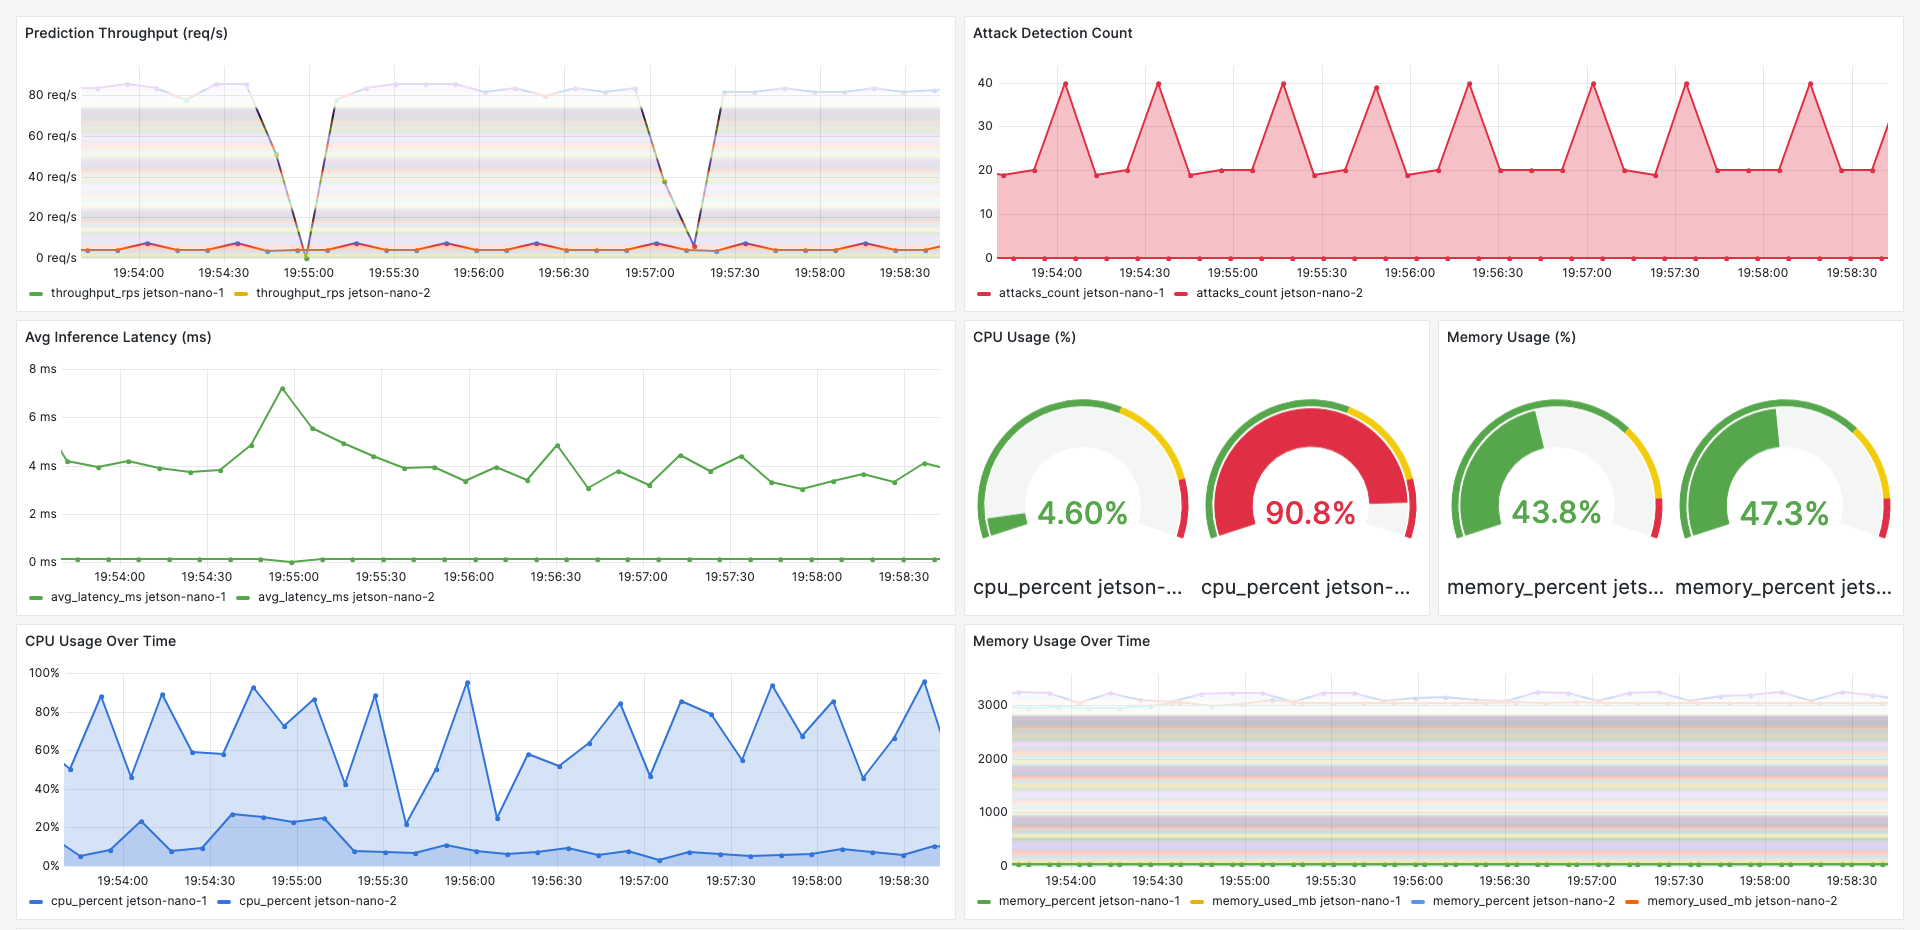
\includegraphics[width=\textwidth]{grafana_peak_load.png}
    \end{column}
    \begin{column}{0.35\textwidth}
      Lúc tải cao nhất, chế độ tách tầng:
      \begin{itemize}
        \item bo cổng lọc: \good{4,6\% CPU}
        \item bo phân loại: \bad{90,8\% CPU}
      \end{itemize}
      \vspace{0.5em}
      Bộ phân loại chiếm gần hết sức tính --- nên tách nó ra khỏi đường nhận
      dữ liệu là đáng.
    \end{column}
  \end{columns}
  \note{Ảnh Grafana chụp khi đang phát lại dữ liệu ở chế độ tách tầng.}
\end{frame}

% ---------------------------------------------------------------- 0:45
\begin{frame}{Kết quả 3: năng lượng mỗi phán quyết giảm từ 2,5 J còn 0,18 J}
  \begin{columns}[T]
    \begin{column}{0.46\textwidth}
      \centering\small
      \fitwidth{%
      \begin{tabular}{lc}
        \toprule
        Cách triển khai & J / phán quyết \\
        \midrule
        Một bo            & 2,49 \\
        \textbf{A: Tách tầng} & \num{0,18} \\
        B: Nhân bản       & 2,25 \\
        C: Cụm Spark      & 0,12 \\
        \bottomrule
      \end{tabular}
      }
    \end{column}
    \begin{column}{0.51\textwidth}
      \begin{itemize}\small
        \setlength{\itemsep}{0.4em}
        \item Ở 100 luồng/giây, điện năng \emph{tăng thêm} khi chạy quá nhỏ
              để đo ($<$0,15\,W).
        \item Nên con số chủ yếu là \key{điện nền của bo chia đều cho số phán
              quyết}.
        \item Tách tầng và cụm Spark ra nhiều phán quyết hơn 24--35 lần, nên
              mỗi phán quyết tốn ít hơn hẳn.
      \end{itemize}
    \end{column}
  \end{columns}
  \takeaway{Đây là năng lượng ở \emph{mức triển khai}, không phải năng lượng
  của riêng mô hình.}
  \note{Năng lượng đo bằng tegrastats: 30 giây nền rồi đến cửa sổ tải; chế độ
  hai bo cộng cả hai bo.}
\end{frame}

% ---------------------------------------------------------------- 0:45
\begin{frame}{Kết quả 4: cổng lọc cho lọt bao nhiêu tấn công}
  \begin{columns}[T]
    \begin{column}{0.53\textwidth}
      \centering\small
      \fitwidth{%
      \begin{tabular}{lccc}
        \toprule
        Ngưỡng cổng & Tấn công & Báo & Luồng \\
        (phân vị) & chuyển tiếp & nhầm & bỏ qua \\
        \midrule
        0,99                   & 74,2\% & 1,01\% & 88,0\% \\
        \textbf{0,995 (đang dùng)} & \num{72,3\%} & \num{0,53\%} & 88,7\% \\
        0,999                  & 58,1\% & 0,10\% & 91,2\% \\
        \bottomrule
      \end{tabular}
      }
      \\[0.3em]
      \raggedright\scriptsize Đo offline trên tập kiểm tra CICIDS2017.
    \end{column}
    \begin{column}{0.44\textwidth}
      \begin{itemize}\small
        \setlength{\itemsep}{0.4em}
        \item Luồng bị cổng bỏ qua là \emph{chốt luôn}: \bad{khoảng 28\% luồng
              tấn công} không tới được bộ phân loại.
        \item Hạ ngưỡng thì bắt thêm tấn công nhưng Spark phải xét nhiều luồng
              hơn.
        \item Người vận hành chọn điểm hợp với sức máy.
      \end{itemize}
    \end{column}
  \end{columns}
  \takeaway{Tốc độ gấp 24 lần phải trả bằng recall: cổng là một \key{sự đánh
  đổi có thể chỉnh}, không phải bộ lọc miễn phí.}
  \note{Số liệu từ results/ml\_08\_anomaly\_gate/gate\_operating\_points.csv.
  Tỷ lệ bỏ qua ở đây đo offline trên tập kiểm tra; khi chạy thật cổng bỏ qua
  95,8\% của một mẫu lưu lượng khác, nên hai con số không nhất thiết trùng.
  Đường cong đầy đủ ở slide dự phòng.}
\end{frame}

% ---------------------------------------------------------------- 0:45
\begin{frame}{Kết quả 5: cái giá của việc dùng Spark để suy luận}
  \small Cùng một Random Forest, cùng 29 đặc trưng, cùng một bo --- chỉ đổi
  bộ máy chạy:
  \vspace{0.4em}

  \centering
  \fitwidth{%
  \begin{tabular}{lcccc}
    \toprule
    Bộ máy chạy & Luồng/giây & p95 (ms) & RAM (\%) & mJ mỗi luồng \\
    \midrule
    PySpark (đang dùng) & 22,6    & 532  & 24,3 & 71,6 \\
    scikit-learn        & 204,4   & 49,8 & 13,3 & 2,91 \\
    \textbf{ONNX Runtime} & \num{7870,8} & \num{1,1} & 15,7 & \num{0,06} \\
    \bottomrule
  \end{tabular}
  }
  \\[0.2em]{\scriptsize mJ mỗi luồng: năng lượng tăng thêm so với lúc bo nghỉ.}
  \takeaway{ONNX Runtime nhanh gấp \num{348 lần} PySpark. Hướng tiếp theo:
  \key{huấn luyện bằng Spark, suy luận bằng ONNX/TensorRT}.}
  \note{Dùng Spark để suy luận là để cùng một bộ công cụ vừa huấn luyện trên
  cụm vừa chạy trên thiết bị. Cái giá là JVM: scikit-learn đã nhanh gấp 9 lần,
  p95 thấp hơn khoảng 11 lần, RAM bằng khoảng nửa. Đo ở batch 10, năng lượng
  tăng thêm tại mức bão hòa.}
\end{frame}

% ---------------------------------------------------------------- 0:40
\begin{frame}{Kết luận}
  \begin{columns}[T]
    \begin{column}{0.55\textwidth}
      \textbf{Những gì đã chỉ ra}
      \begin{itemize}\small
        \setlength{\itemsep}{0.3em}
        \item Tách cổng lọc và bộ phân loại ra hai bo: \good{2,6 $\rightarrow$
              62,5 phán quyết/giây}, p95 $\approx$13\,ms.
        \item Năng lượng mỗi phán quyết: \good{2,5\,J $\rightarrow$ 0,18\,J}.
        \item Đổi lại, cổng cho lọt \bad{$\approx$28\%} luồng tấn công ở ngưỡng
              đang dùng.
        \item Spark là nút thắt suy luận: ONNX nhanh gấp 348 lần.
      \end{itemize}
    \end{column}
    \begin{column}{0.42\textwidth}
      \textbf{Hạn chế}
      \begin{itemize}\footnotesize
        \item Hai bo, mạng Wi-Fi, dữ liệu phát lại.
        \item GPU chưa dùng; chưa thử tấn công né tránh.
      \end{itemize}
      \textbf{Hướng tiếp theo}
      \begin{itemize}\footnotesize
        \item Suy luận bằng ONNX/TensorRT.
        \item Lưu lượng thật; huấn luyện lại khi dữ liệu trôi.
      \end{itemize}
    \end{column}
  \end{columns}
  \vfill
  \centering \key{Xin cảm ơn --- kính mời câu hỏi}
  \note{Nhắc lại ba con số: gấp 24 lần, 13 mili giây, 0,18 J. Và nói thẳng cái
  giá: khoảng 28\% luồng tấn công bị cổng cho qua ở ngưỡng hiện tại.}
\end{frame}

% ---------------------------------------------------------------- ~11:00
\begin{frame}{Tài liệu tham khảo chính}
  \begin{itemize}\footnotesize
    \setlength{\itemsep}{0em}
    \item[{[1]}] Sharafaldin, I., Lashkari, A.\,H. \& Ghorbani, A.\,A.
          \emph{Toward generating a new intrusion detection dataset and
          intrusion traffic characterization}. ICISSP 2018.
          \hfill{\key{CICIDS2017}}
    \item[{[2]}] Shi, W. et al. \emph{Edge computing: Vision and challenges}.
          IEEE Internet of Things Journal 3(5), 2016.
          \hfill{\key{điện toán biên}}
    \item[{[3]}] Chandola, V., Banerjee, A. \& Kumar, V. \emph{Anomaly detection:
          A survey}. ACM Computing Surveys 41(3), 2009.
          \hfill{\key{cổng lọc}}
    \item[{[4]}] Lundberg, S.\,M. \& Lee, S.-I. \emph{A unified approach to
          interpreting model predictions}. NeurIPS 2017.
          \hfill{\key{SHAP}}
    \item[{[5]}] Zaharia, M. et al. \emph{Spark: Cluster computing with working
          sets}. HotCloud 2010.
          \hfill{\key{Spark}}
    \item[{[6]}] Kreps, J., Narkhede, N. \& Rao, J. \emph{Kafka: a Distributed
          Messaging System for Log Processing}. NetDB 2011.
          \hfill{\key{Kafka}}
    \item[{[7]}] Mohan Kiran Kumar, K. et al. \emph{Distributed Intrusion Detection
          System using Kafka and Spark Streaming}. ICVADV 2025.
          \hfill{\key{hệ thống gần nhất}}
    \item[{[8]}] Arp, D. et al. \emph{Dos and Don'ts of Machine Learning in Computer
          Security}. USENIX Security 2022.
          \hfill{\key{chống rò rỉ}}
  \end{itemize}
\end{frame}

% =====================================================================
\appendix

\begin{frame}[standout]
  Slide dự phòng
\end{frame}

\begin{frame}{Dự phòng: biểu đồ so sánh các cách triển khai}
  \centering
  \IfFileExists{../../papers/soict2026/results/benchmarks/edge_modes.png}
    {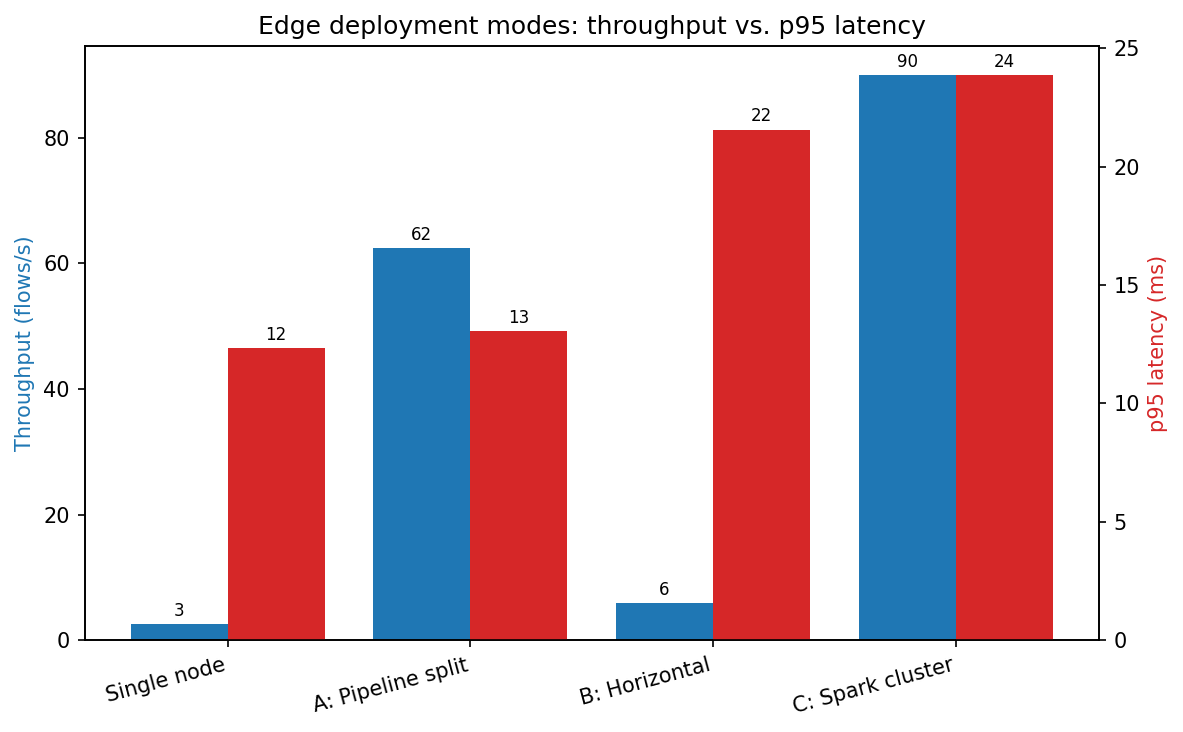
\includegraphics[height=0.72\textheight, width=\textwidth, keepaspectratio]{edge_modes.png}}
    {\fbox{\parbox{0.7\textwidth}{\centering\vspace{1.5cm}
      \texttt{edge\_modes.png}\vspace{1.5cm}}}}
  \\[0.2em]
  \footnotesize Số phán quyết mỗi giây (trái) và độ trễ p95 (phải).
\end{frame}

\begin{frame}{Dự phòng: đường cong vận hành của cổng lọc}
  \centering
  \IfFileExists{../../results/ml_08_anomaly_gate/gate_operating_points.png}
    {\includegraphics[height=0.68\textheight, width=\textwidth, keepaspectratio]{gate_operating_points.png}}
    {\fbox{\parbox{0.7\textwidth}{\centering\vspace{1.5cm}
      \texttt{gate\_operating\_points.png}\vspace{1.5cm}}}}
  \\[0.2em]
  \footnotesize Recall tấn công (trái) và tỷ lệ báo nhầm (phải) theo tỷ lệ luồng
  bị bỏ qua. Bỏ qua nhiều hơn thì Spark nhẹ hơn nhưng lọt nhiều tấn công hơn.
\end{frame}

\begin{frame}{Dự phòng: bảng điều khiển giám sát đầy đủ}
  \centering
  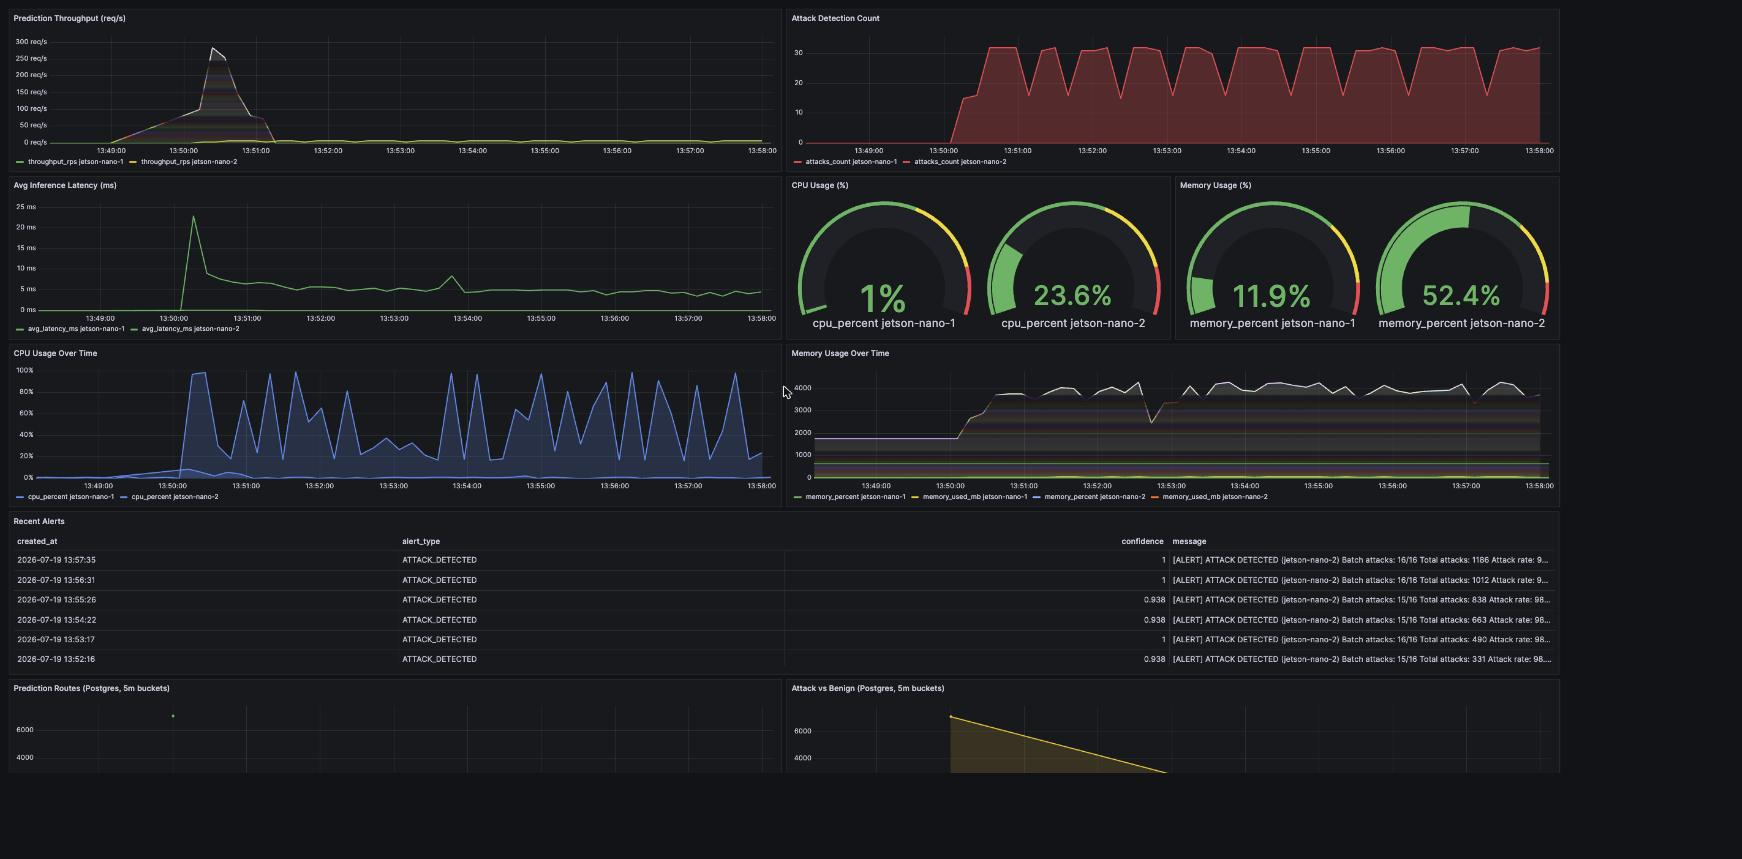
\includegraphics[height=0.70\textheight, width=\textwidth, keepaspectratio]{grafana_dashboard.png}
  \\[0.2em]
  \footnotesize Tốc độ từng bo, số tấn công phát hiện, độ trễ suy luận, CPU/RAM
  hai bo, cảnh báo lưu trong PostgreSQL.
\end{frame}

\begin{frame}{Dự phòng: quy trình đo}
  \begin{itemize}\small
    \item Máy chủ khởi động các vai trò trên Jetson qua SSH, tạo tải, thu log
          từng bo.
    \item Mỗi cấu hình lặp $\geq$3 lần; bỏ giai đoạn khởi động để JVM chưa
          nóng máy không làm phồng số liệu.
    \item Truy vấn chỉ số khớp đúng cửa sổ tải, không lấy khoảng thời gian trượt.
    \item p95 tính theo từng bo trên dữ liệu thô của từng luồng; p95 của cụm lấy
          bo tệ nhất.
    \item Độ trễ đầu cuối tính từ lúc gửi tới lúc có phán quyết, đồng hồ đồng bộ
          NTP, không tính thời gian ghi CSDL.
    \item Năng lượng: \texttt{tegrastats}, 30 giây nền rồi cửa sổ tải; chế độ
          hai bo cộng cả hai bo.
  \end{itemize}
\end{frame}

\end{document}
"
% ---------------------------------------------------------------------
\ifdefined\shownotes
  \usepackage{pgfpages}
  \setbeameroption{show notes on second screen=right}
\fi

\centeredtitles

\graphicspath{%
  {../../papers/soict2026/results/benchmarks/}%
  {../../papers/soict2026/figures/}%
  {../../results/ml_08_anomaly_gate/}%
  {../../results/ml_07_cross_method_comparison/}%
}

\title{Hệ thống phát hiện xâm nhập phân tán thời gian thực trên cụm thiết bị biên Jetson Orin Nano Super với Kafka và PySpark}
\author{\textbf{Nguyễn Vũ Thái}\inst{1} \and Bùi Văn Dũng\inst{2} \and Đỗ Trí Nhựt\inst{2} \and Nguyễn Văn Dũ\inst{3}}
\institute{\scriptsize
           \inst{1}Phân hiệu tại TP.\ Hồ Chí Minh, Trường Đại học Giao thông Vận tải, TP.\ Hồ Chí Minh, Việt Nam \\
           \inst{2}Trường Đại học Công nghệ Thông tin, ĐHQG-HCM, TP.\ Hồ Chí Minh, Việt Nam \\
           \inst{3}Khoa Công nghệ Thông tin, Trường Đại học Nông Lâm, TP.\ Hồ Chí Minh, Việt Nam}
\date{SOICT 2026}

\begin{document}

% ---------------------------------------------------------------- 0:20
\maketitle
\note{Câu hỏi của bài: có hai bo mạch biên thì nên chia việc phát hiện xâm nhập
giữa chúng thế nào, và bo thứ hai thực sự đem lại bao nhiêu.}

% =====================================================================
\section{I.\ VẤN ĐỀ VÀ ĐÓNG GÓP}
% =====================================================================

% ---------------------------------------------------------------- 0:45
\begin{frame}{Phát hiện xâm nhập ngay tại thiết bị biên: còn ba khoảng trống}
  \begin{columns}[T]
    \begin{column}{0.55\textwidth}
      Mô hình phát hiện xâm nhập nay đã \emph{chạy được} trên bo mạch nhỏ, nhưng
      nếu một bo phải xét \key{mọi} luồng thì nó quá tải rất nhanh.
      \vspace{0.6em}

      \textbf{Nghiên cứu trước còn thiếu}
      \begin{enumerate}
        \item Chỉ đo trên \bad{một thiết bị}, không chia việc cho nhiều bo.
        \item Hiếm khi báo \bad{cùng lúc} tốc độ, độ trễ và năng lượng.
        \item Điểm số offline lấy từ quy trình \bad{rò rỉ dữ liệu}.
      \end{enumerate}
    \end{column}
    \begin{column}{0.40\textwidth}
      \begin{alertblock}{Câu hỏi}
        Có hai bo Jetson thì nên \emph{đặt} việc phát hiện lên chúng thế nào?
      \end{alertblock}
      \begin{exampleblock}{Cách làm}
        Tách làm hai: \key{cổng lọc} rẻ trên bo \#1, \key{bộ phân loại}
        nặng trên bo \#2, nối bằng Kafka.
      \end{exampleblock}
    \end{column}
  \end{columns}
  \note{Khoảng trống thứ ba là lý do nhóm làm bài FAIR về quy trình đánh giá
  chống rò rỉ.}
\end{frame}

% ---------------------------------------------------------------- 0:30
\begin{frame}{Các đóng góp}
  \begin{enumerate}
    \setlength{\itemsep}{0.4em}
    \item Hệ thống phát hiện xâm nhập \key{hai tầng, phân tán}: cổng lọc và
          bộ phân loại Spark đặt trên hai bo khác nhau.
    \item \key{Ba cách triển khai} trên cụm hai Jetson: tách tầng, nhân bản
          ngang, cụm Spark.
    \item \key{Đo đầu cuối}: tốc độ, độ trễ, CPU/RAM từng bo \emph{và} năng
          lượng mỗi phán quyết.
    \item Mã nguồn, cấu hình và kịch bản đo \key{công khai}, chạy lại được.
  \end{enumerate}
  \note{Phán quyết (verdict) là quyết định cuối cùng bình thường hay tấn công
  cho một luồng.}
\end{frame}

% =====================================================================
\section{II.\ HỆ THỐNG VÀ CÁCH ĐO}
% =====================================================================

% ---------------------------------------------------------------- 0:50
\begin{frame}{Kiến trúc: tách cổng lọc và bộ phân loại ra hai bo}
  \centering
  \resizebox{0.72\textwidth}{!}{%
  \begin{tikzpicture}[
      font=\small, >=Stealth, every node/.style={align=center},
      pc/.style ={draw=gray!60, thick, rounded corners, fill=gray!8, minimum width=13.4cm, minimum height=1.25cm, inner sep=3pt},
      jet/.style={draw=accGreen!80!black, thick, rounded corners, fill=accGreen!8, text width=4.4cm, minimum height=1.9cm, inner sep=4pt},
      mtr/.style={draw=accBlue, thick, rounded corners, fill=accBlue!5, minimum width=13.4cm, minimum height=0.95cm, inner sep=3pt},
      lbl/.style={font=\footnotesize, fill=white, inner sep=1.5pt, align=center, text=accBlue!75!black},
      arr/.style={-{Stealth[length=2.5mm]}, thick, draw=gray!60!black},
      dsh/.style={-{Stealth[length=2.5mm]}, thick, draw=accBlue, dashed},
  ]
    \node[pc]  (pc)  at (0, 0.0)   {\textbf{Máy chủ điều phối (PC, Docker)}\\[2pt]
        Kafka \;$|$\; PostgreSQL \;$|$\; InfluxDB \;$|$\; Grafana \;$|$\; phát lại luồng CSV};
    \node[jet] (j1)  at (-4.6,-3.2) {\textbf{Jetson \#1}\\[2pt] \key{Cổng lọc}\\[2pt]
        Autoencoder bỏ qua luồng bình thường};
    \node[jet] (j2)  at ( 4.6,-3.2) {\textbf{Jetson \#2}\\[2pt] \key{Bộ phân loại}\\[2pt]
        PySpark: bình thường / tấn công};
    \node[mtr] (out) at (0,-6.0)   {Chỉ số hiệu năng $\rightarrow$ InfluxDB $\rightarrow$ Grafana \quad$|$\quad
        Cảnh báo: Email / Slack};
    \draw[arr] (pc.south -| j1) -- node[lbl]{luồng mạng} (j1.north);
    \draw[arr] (j1.east) -- node[lbl]{chỉ luồng đáng ngờ\\ ($\approx$4\% số luồng)} (j2.west);
    \draw[arr] (j2.north) -- node[lbl]{kết quả\\ $\rightarrow$ PostgreSQL} (pc.south -| j2);
    \draw[dsh] (j1.south) -- (out.north -| j1);
    \draw[dsh] (j2.south) -- (out.north -| j2);
  \end{tikzpicture}}
  \\[0.3em]
  \small Chỉ các luồng đáng ngờ mới đi qua Kafka sang bo \#2.
  \note{Máy chủ chạy hạ tầng. Bo một lọc, bo hai phân loại. Mọi chỉ số đi vào
  Grafana theo thời gian thực.}
\end{frame}

% ---------------------------------------------------------------- 0:50
\begin{frame}{Hai tầng làm việc thế nào}
  \begin{columns}[T]
    \begin{column}{0.49\textwidth}
      \textbf{Tầng 1 --- cổng lọc (autoencoder)}
      \begin{itemize}\small
        \item Học cách \emph{tái tạo} lưu lượng bình thường.
        \item Luồng tái tạo tốt (sai số nhỏ) $\rightarrow$ coi là bình thường,
              \key{dừng luôn}.
        \item Luồng tái tạo kém $\rightarrow$ đáng ngờ, chuyển sang tầng 2.
        \item Ngưỡng sai số chọn \emph{trước} trên 10\% dữ liệu bình thường,
              không nhìn tập kiểm tra.
      \end{itemize}
    \end{column}
    \begin{column}{0.49\textwidth}
      \textbf{Tầng 2 --- bộ phân loại (PySpark)}
      \begin{itemize}\small
        \item Random Forest trên \key{29 đặc trưng} được SHAP chọn,
              không có cổng đích.
        \item Chỉ phải xét số ít luồng mà cổng chuyển sang.
      \end{itemize}
    \end{column}
  \end{columns}
  \note{Sai số tái tạo là MSE. Ngưỡng là phân vị 0,995 của MSE trên tập kiểm
  định gồm 10\% luồng bình thường của tập huấn luyện
  (jetson/model/anomaly\_threshold.json). Bộ 29 đặc trưng
  (jetson/model/feature\_columns.json) lấy từ một bảng xếp hạng SHAP \emph{cũ}
  đã bỏ destination\_port; nó chỉ trùng 15/30 với SHAP Top-30 hiện tại của bài
  FAIR, xem jetson/config.py.}
\end{frame}

% ---------------------------------------------------------------- 0:40
\begin{frame}{Vì sao bộ phân loại là Random Forest trên Spark}
  \begin{itemize}
    \setlength{\itemsep}{0.5em}
    \item \key{Random Forest có sẵn trong Spark ML}, nên mô hình xuất ra chạy
          được trên Jetson (ARM64) mà không cần thư viện native như XGBoost.
    \item \key{Ít đặc trưng} (29 thay vì 77) thì dựng vector và suy luận nhanh
          hơn trên bo 8\,GB.
    \item \key{Cùng một bộ công cụ} (Spark) vừa huấn luyện trên cụm vừa chạy
          trên thiết bị --- cái giá của lựa chọn này ở Kết quả 5.
  \end{itemize}
  \note{Bộ 29 đặc trưng của mô hình đang chạy lấy từ một bảng xếp hạng SHAP cũ,
  không phải SHAP Top-30 hiện tại của bài FAIR (chỉ trùng 15/30). Vì vậy slide
  này không trích F1 0,9955 của bài FAIR cho mô hình triển khai. Các số đo tốc
  độ, độ trễ, năng lượng vẫn là của đúng mô hình đang chạy.}
\end{frame}

% ---------------------------------------------------------------- 0:50
\begin{frame}{Ba cách triển khai, cùng một khối lượng việc}
  \begin{columns}[T]
    \begin{column}{0.56\textwidth}
      \begin{description}\small
        \item[Một bo] làm hết mọi việc --- mốc so sánh.
        \item[A: Tách tầng] cổng trên \#1, phân loại trên \#2.
        \item[B: Nhân bản] mỗi bo làm \emph{đủ} cả hai tầng, chia nhau luồng
              qua Kafka.
        \item[C: Cụm Spark] PC làm master, hai bo làm worker.
      \end{description}
      \vspace{0.3em}
      \footnotesize Tốc độ tính bằng \key{số phán quyết mỗi giây}: một luồng
      được quyết ở cổng \emph{hoặc} ở bộ phân loại, không đếm hai lần.
    \end{column}
    \begin{column}{0.41\textwidth}
      \begin{block}{Thiết lập đo}
        \footnotesize
        2$\times$ Jetson Orin Nano Super: CPU 6 nhân, 8\,GB RAM, GPU $\approx$67 TOPS\\[0.3em]
        PySpark 3.4.1, Kafka 3.5, mạng Wi-Fi\\[0.3em]
        Phát lại CICIDS2017, 100 luồng/giây\\[0.3em]
        Mỗi cấu hình lặp $\geq$3 lần, bỏ giai đoạn khởi động\\[0.3em]
        Năng lượng đo bằng \texttt{tegrastats}
      \end{block}
    \end{column}
  \end{columns}
  \note{Độ trễ p95 tính theo từng bo trên dữ liệu thô của từng luồng, và lấy bo
  tệ nhất làm con số của cả cụm. Bỏ giai đoạn khởi động để JVM chưa nóng máy
  không làm phồng độ trễ.}
\end{frame}

% =====================================================================
\section{III.\ KẾT QUẢ VÀ KẾT LUẬN}
% =====================================================================

% ---------------------------------------------------------------- 1:00
\begin{frame}{Kết quả 1: tách tầng nhanh gấp 24 lần, độ trễ gần như không đổi}
  \begin{columns}[T]
    \begin{column}{0.54\textwidth}
      \centering\small
      \fitwidth{%
      \begin{tabular}{lcc}
        \toprule
        Cách triển khai & Phán quyết/giây & Độ trễ p95 (ms) \\
        \midrule
        Một bo            & 2,6            & 12,3 \\
        \textbf{A: Tách tầng} & \num{62,5} & \num{13,1} \\
        B: Nhân bản       & 5,9            & 21,6 \\
        C: Cụm Spark      & 90,0           & 23,9 \\
        \bottomrule
      \end{tabular}
      }
      \\[0.3em]
      \raggedright\scriptsize \textbf{p95}: 95\% số luồng có phán quyết nhanh
      hơn mức này.
    \end{column}
    \begin{column}{0.43\textwidth}
      \begin{itemize}
        \setlength{\itemsep}{0.4em}
        \item \good{Tách tầng: gấp 24 lần}, cổng xử lý xong 95,8\% số luồng
              trước khi tới Spark.
        \item \bad{Nhân bản: chỉ gấp 2,3 lần} --- bo nào cũng vẫn phải chạy
              Spark.
        \item Cụm Spark nhanh nhất nhưng \bad{dao động mạnh} ($\pm$25,6).
      \end{itemize}
    \end{column}
  \end{columns}
  \takeaway{\textbf{Nên dùng tách tầng}: nhanh và ổn định nhất.}
  \note{Độ lệch giữa các lần lặp: một bo 2,60 $\pm$ 0,41; tách tầng 62,5
  $\pm$ 0,6; nhân bản 5,9 $\pm$ 1,4; cụm Spark 90,0 $\pm$ 25,6 luồng/giây. Độ
  trễ p95 lệch 3,0 / 2,6 / 19,2 / 17,8 ms. Nhân bản chứng minh lợi ích đến từ
  việc tách vai trò, không phải từ việc thêm một bo. Cụm Spark còn cần thêm máy
  master và hợp với mô hình quá lớn cho một bo.}
\end{frame}

% ---------------------------------------------------------------- 0:35
\begin{frame}{Kết quả 2: nhìn trực tiếp thấy bo nào đang gánh việc}
  \begin{columns}[c]
    \begin{column}{0.63\textwidth}
      \centering
      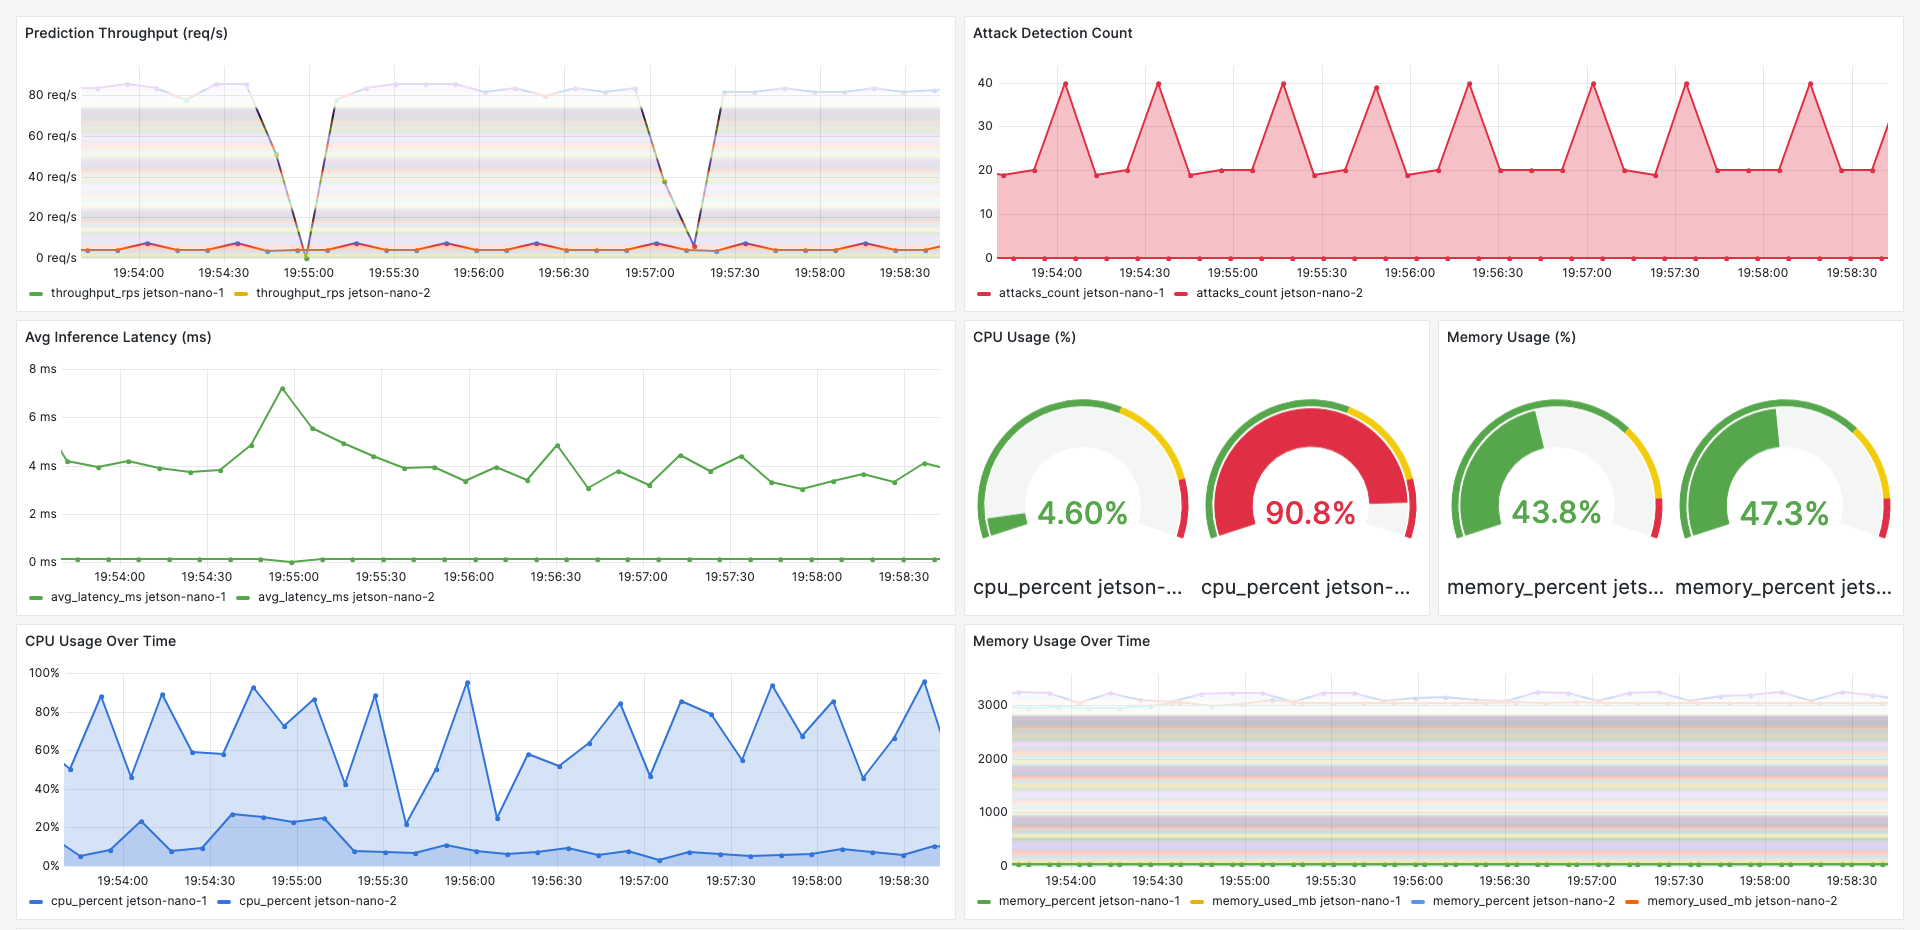
\includegraphics[width=\textwidth]{grafana_peak_load.png}
    \end{column}
    \begin{column}{0.35\textwidth}
      Lúc tải cao nhất, chế độ tách tầng:
      \begin{itemize}
        \item bo cổng lọc: \good{4,6\% CPU}
        \item bo phân loại: \bad{90,8\% CPU}
      \end{itemize}
      \vspace{0.5em}
      Bộ phân loại chiếm gần hết sức tính --- nên tách nó ra khỏi đường nhận
      dữ liệu là đáng.
    \end{column}
  \end{columns}
  \note{Ảnh Grafana chụp khi đang phát lại dữ liệu ở chế độ tách tầng.}
\end{frame}

% ---------------------------------------------------------------- 0:45
\begin{frame}{Kết quả 3: năng lượng mỗi phán quyết giảm từ 2,5 J còn 0,18 J}
  \begin{columns}[T]
    \begin{column}{0.46\textwidth}
      \centering\small
      \fitwidth{%
      \begin{tabular}{lc}
        \toprule
        Cách triển khai & J / phán quyết \\
        \midrule
        Một bo            & 2,49 \\
        \textbf{A: Tách tầng} & \num{0,18} \\
        B: Nhân bản       & 2,25 \\
        C: Cụm Spark      & 0,12 \\
        \bottomrule
      \end{tabular}
      }
    \end{column}
    \begin{column}{0.51\textwidth}
      \begin{itemize}\small
        \setlength{\itemsep}{0.4em}
        \item Ở 100 luồng/giây, điện năng \emph{tăng thêm} khi chạy quá nhỏ
              để đo ($<$0,15\,W).
        \item Nên con số chủ yếu là \key{điện nền của bo chia đều cho số phán
              quyết}.
        \item Tách tầng và cụm Spark ra nhiều phán quyết hơn 24--35 lần, nên
              mỗi phán quyết tốn ít hơn hẳn.
      \end{itemize}
    \end{column}
  \end{columns}
  \takeaway{Đây là năng lượng ở \emph{mức triển khai}, không phải năng lượng
  của riêng mô hình.}
  \note{Năng lượng đo bằng tegrastats: 30 giây nền rồi đến cửa sổ tải; chế độ
  hai bo cộng cả hai bo.}
\end{frame}

% ---------------------------------------------------------------- 0:45
\begin{frame}{Kết quả 4: cổng lọc cho lọt bao nhiêu tấn công}
  \begin{columns}[T]
    \begin{column}{0.53\textwidth}
      \centering\small
      \fitwidth{%
      \begin{tabular}{lccc}
        \toprule
        Ngưỡng cổng & Tấn công & Báo & Luồng \\
        (phân vị) & chuyển tiếp & nhầm & bỏ qua \\
        \midrule
        0,99                   & 74,2\% & 1,01\% & 88,0\% \\
        \textbf{0,995 (đang dùng)} & \num{72,3\%} & \num{0,53\%} & 88,7\% \\
        0,999                  & 58,1\% & 0,10\% & 91,2\% \\
        \bottomrule
      \end{tabular}
      }
      \\[0.3em]
      \raggedright\scriptsize Đo offline trên tập kiểm tra CICIDS2017.
    \end{column}
    \begin{column}{0.44\textwidth}
      \begin{itemize}\small
        \setlength{\itemsep}{0.4em}
        \item Luồng bị cổng bỏ qua là \emph{chốt luôn}: \bad{khoảng 28\% luồng
              tấn công} không tới được bộ phân loại.
        \item Hạ ngưỡng thì bắt thêm tấn công nhưng Spark phải xét nhiều luồng
              hơn.
        \item Người vận hành chọn điểm hợp với sức máy.
      \end{itemize}
    \end{column}
  \end{columns}
  \takeaway{Tốc độ gấp 24 lần phải trả bằng recall: cổng là một \key{sự đánh
  đổi có thể chỉnh}, không phải bộ lọc miễn phí.}
  \note{Số liệu từ results/ml\_08\_anomaly\_gate/gate\_operating\_points.csv.
  Tỷ lệ bỏ qua ở đây đo offline trên tập kiểm tra; khi chạy thật cổng bỏ qua
  95,8\% của một mẫu lưu lượng khác, nên hai con số không nhất thiết trùng.
  Đường cong đầy đủ ở slide dự phòng.}
\end{frame}

% ---------------------------------------------------------------- 0:45
\begin{frame}{Kết quả 5: cái giá của việc dùng Spark để suy luận}
  \small Cùng một Random Forest, cùng 29 đặc trưng, cùng một bo --- chỉ đổi
  bộ máy chạy:
  \vspace{0.4em}

  \centering
  \fitwidth{%
  \begin{tabular}{lcccc}
    \toprule
    Bộ máy chạy & Luồng/giây & p95 (ms) & RAM (\%) & mJ mỗi luồng \\
    \midrule
    PySpark (đang dùng) & 22,6    & 532  & 24,3 & 71,6 \\
    scikit-learn        & 204,4   & 49,8 & 13,3 & 2,91 \\
    \textbf{ONNX Runtime} & \num{7870,8} & \num{1,1} & 15,7 & \num{0,06} \\
    \bottomrule
  \end{tabular}
  }
  \\[0.2em]{\scriptsize mJ mỗi luồng: năng lượng tăng thêm so với lúc bo nghỉ.}
  \takeaway{ONNX Runtime nhanh gấp \num{348 lần} PySpark. Hướng tiếp theo:
  \key{huấn luyện bằng Spark, suy luận bằng ONNX/TensorRT}.}
  \note{Dùng Spark để suy luận là để cùng một bộ công cụ vừa huấn luyện trên
  cụm vừa chạy trên thiết bị. Cái giá là JVM: scikit-learn đã nhanh gấp 9 lần,
  p95 thấp hơn khoảng 11 lần, RAM bằng khoảng nửa. Đo ở batch 10, năng lượng
  tăng thêm tại mức bão hòa.}
\end{frame}

% ---------------------------------------------------------------- 0:40
\begin{frame}{Kết luận}
  \begin{columns}[T]
    \begin{column}{0.55\textwidth}
      \textbf{Những gì đã chỉ ra}
      \begin{itemize}\small
        \setlength{\itemsep}{0.3em}
        \item Tách cổng lọc và bộ phân loại ra hai bo: \good{2,6 $\rightarrow$
              62,5 phán quyết/giây}, p95 $\approx$13\,ms.
        \item Năng lượng mỗi phán quyết: \good{2,5\,J $\rightarrow$ 0,18\,J}.
        \item Đổi lại, cổng cho lọt \bad{$\approx$28\%} luồng tấn công ở ngưỡng
              đang dùng.
        \item Spark là nút thắt suy luận: ONNX nhanh gấp 348 lần.
      \end{itemize}
    \end{column}
    \begin{column}{0.42\textwidth}
      \textbf{Hạn chế}
      \begin{itemize}\footnotesize
        \item Hai bo, mạng Wi-Fi, dữ liệu phát lại.
        \item GPU chưa dùng; chưa thử tấn công né tránh.
      \end{itemize}
      \textbf{Hướng tiếp theo}
      \begin{itemize}\footnotesize
        \item Suy luận bằng ONNX/TensorRT.
        \item Lưu lượng thật; huấn luyện lại khi dữ liệu trôi.
      \end{itemize}
    \end{column}
  \end{columns}
  \vfill
  \centering \key{Xin cảm ơn --- kính mời câu hỏi}
  \note{Nhắc lại ba con số: gấp 24 lần, 13 mili giây, 0,18 J. Và nói thẳng cái
  giá: khoảng 28\% luồng tấn công bị cổng cho qua ở ngưỡng hiện tại.}
\end{frame}

% ---------------------------------------------------------------- ~11:00
\begin{frame}{Tài liệu tham khảo chính}
  \begin{itemize}\footnotesize
    \setlength{\itemsep}{0em}
    \item[{[1]}] Sharafaldin, I., Lashkari, A.\,H. \& Ghorbani, A.\,A.
          \emph{Toward generating a new intrusion detection dataset and
          intrusion traffic characterization}. ICISSP 2018.
          \hfill{\key{CICIDS2017}}
    \item[{[2]}] Shi, W. et al. \emph{Edge computing: Vision and challenges}.
          IEEE Internet of Things Journal 3(5), 2016.
          \hfill{\key{điện toán biên}}
    \item[{[3]}] Chandola, V., Banerjee, A. \& Kumar, V. \emph{Anomaly detection:
          A survey}. ACM Computing Surveys 41(3), 2009.
          \hfill{\key{cổng lọc}}
    \item[{[4]}] Lundberg, S.\,M. \& Lee, S.-I. \emph{A unified approach to
          interpreting model predictions}. NeurIPS 2017.
          \hfill{\key{SHAP}}
    \item[{[5]}] Zaharia, M. et al. \emph{Spark: Cluster computing with working
          sets}. HotCloud 2010.
          \hfill{\key{Spark}}
    \item[{[6]}] Kreps, J., Narkhede, N. \& Rao, J. \emph{Kafka: a Distributed
          Messaging System for Log Processing}. NetDB 2011.
          \hfill{\key{Kafka}}
    \item[{[7]}] Mohan Kiran Kumar, K. et al. \emph{Distributed Intrusion Detection
          System using Kafka and Spark Streaming}. ICVADV 2025.
          \hfill{\key{hệ thống gần nhất}}
    \item[{[8]}] Arp, D. et al. \emph{Dos and Don'ts of Machine Learning in Computer
          Security}. USENIX Security 2022.
          \hfill{\key{chống rò rỉ}}
  \end{itemize}
\end{frame}

% =====================================================================
\appendix

\begin{frame}[standout]
  Slide dự phòng
\end{frame}

\begin{frame}{Dự phòng: biểu đồ so sánh các cách triển khai}
  \centering
  \IfFileExists{../../papers/soict2026/results/benchmarks/edge_modes.png}
    {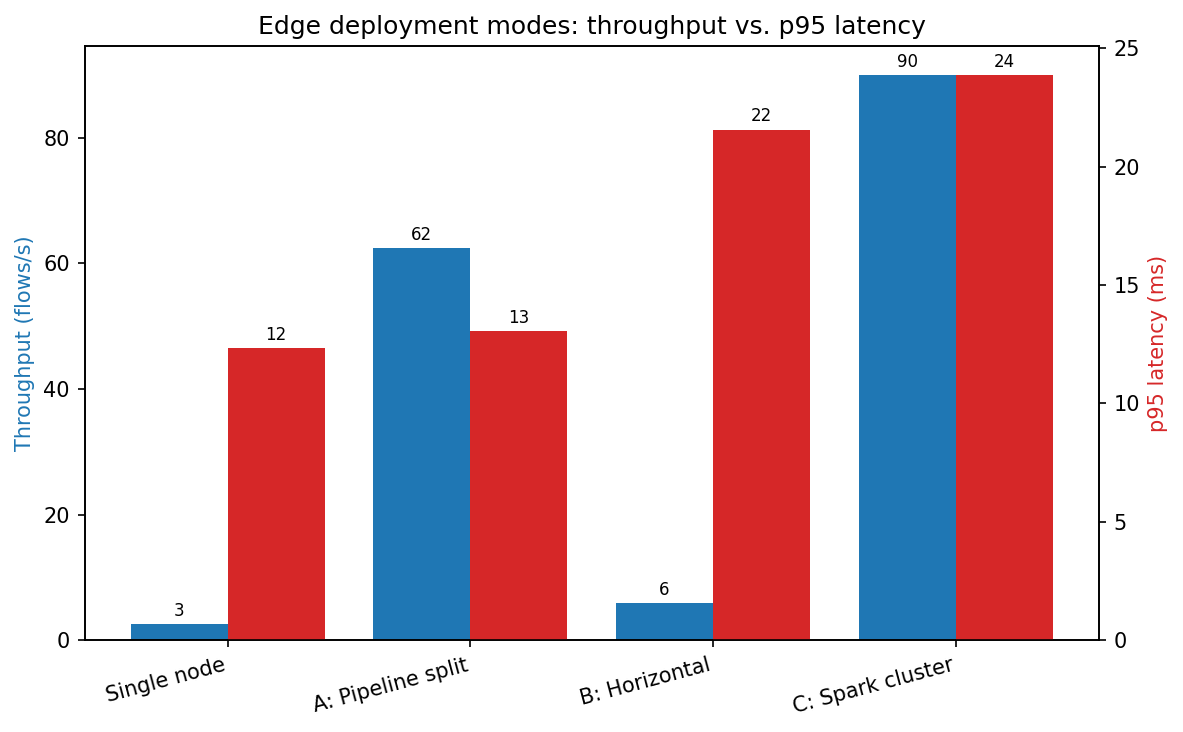
\includegraphics[height=0.72\textheight, width=\textwidth, keepaspectratio]{edge_modes.png}}
    {\fbox{\parbox{0.7\textwidth}{\centering\vspace{1.5cm}
      \texttt{edge\_modes.png}\vspace{1.5cm}}}}
  \\[0.2em]
  \footnotesize Số phán quyết mỗi giây (trái) và độ trễ p95 (phải).
\end{frame}

\begin{frame}{Dự phòng: đường cong vận hành của cổng lọc}
  \centering
  \IfFileExists{../../results/ml_08_anomaly_gate/gate_operating_points.png}
    {\includegraphics[height=0.68\textheight, width=\textwidth, keepaspectratio]{gate_operating_points.png}}
    {\fbox{\parbox{0.7\textwidth}{\centering\vspace{1.5cm}
      \texttt{gate\_operating\_points.png}\vspace{1.5cm}}}}
  \\[0.2em]
  \footnotesize Recall tấn công (trái) và tỷ lệ báo nhầm (phải) theo tỷ lệ luồng
  bị bỏ qua. Bỏ qua nhiều hơn thì Spark nhẹ hơn nhưng lọt nhiều tấn công hơn.
\end{frame}

\begin{frame}{Dự phòng: bảng điều khiển giám sát đầy đủ}
  \centering
  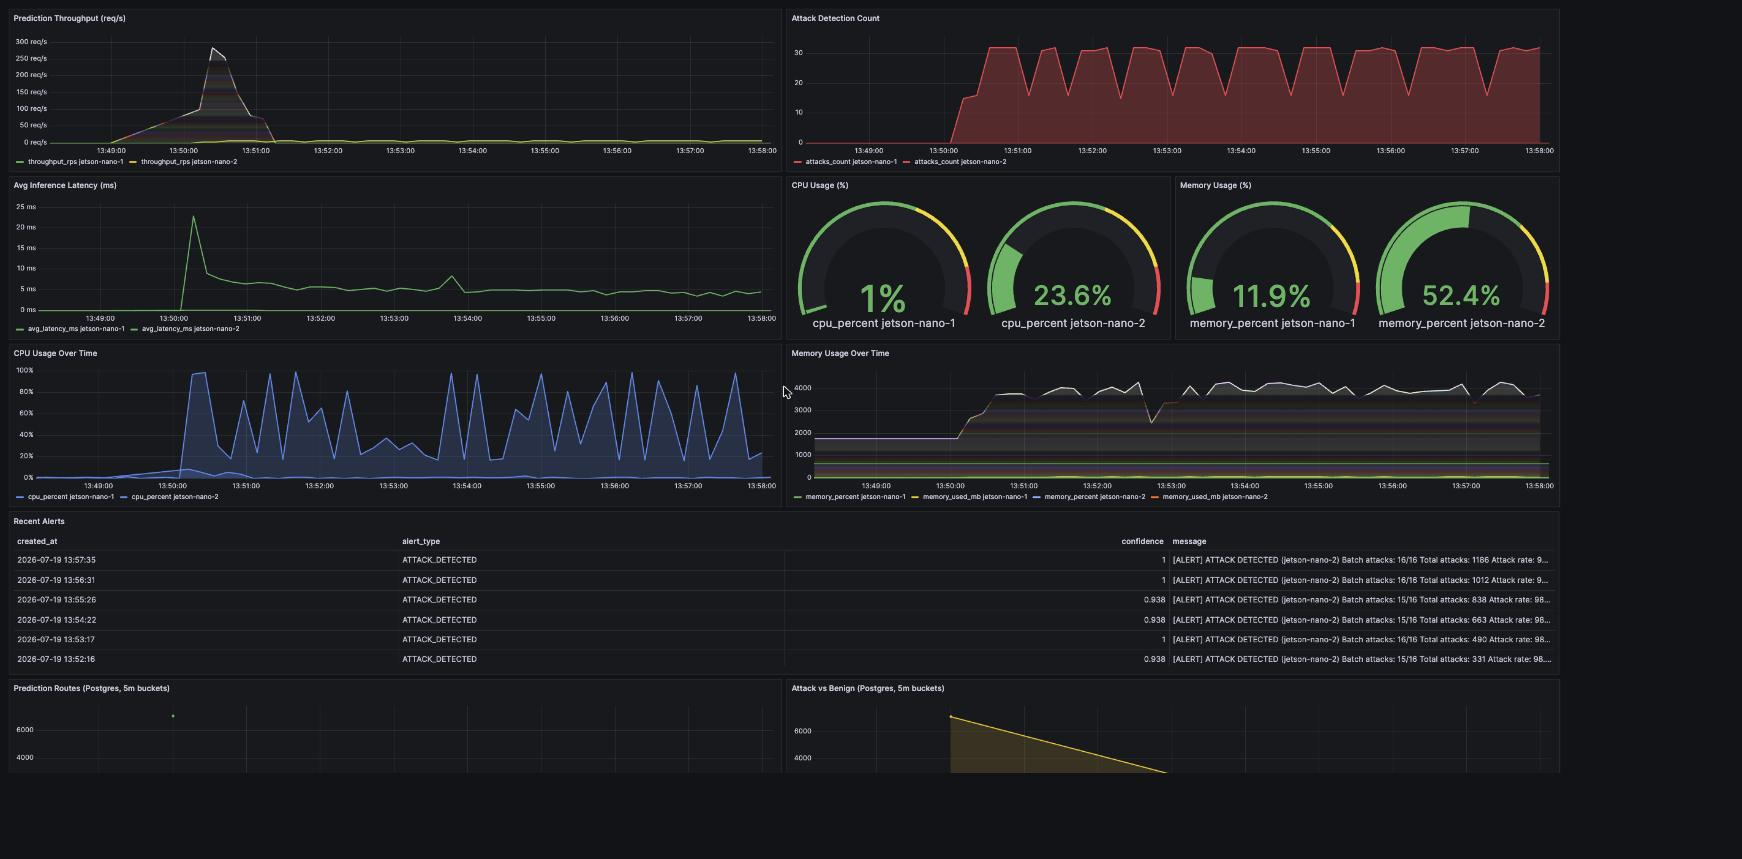
\includegraphics[height=0.70\textheight, width=\textwidth, keepaspectratio]{grafana_dashboard.png}
  \\[0.2em]
  \footnotesize Tốc độ từng bo, số tấn công phát hiện, độ trễ suy luận, CPU/RAM
  hai bo, cảnh báo lưu trong PostgreSQL.
\end{frame}

\begin{frame}{Dự phòng: quy trình đo}
  \begin{itemize}\small
    \item Máy chủ khởi động các vai trò trên Jetson qua SSH, tạo tải, thu log
          từng bo.
    \item Mỗi cấu hình lặp $\geq$3 lần; bỏ giai đoạn khởi động để JVM chưa
          nóng máy không làm phồng số liệu.
    \item Truy vấn chỉ số khớp đúng cửa sổ tải, không lấy khoảng thời gian trượt.
    \item p95 tính theo từng bo trên dữ liệu thô của từng luồng; p95 của cụm lấy
          bo tệ nhất.
    \item Độ trễ đầu cuối tính từ lúc gửi tới lúc có phán quyết, đồng hồ đồng bộ
          NTP, không tính thời gian ghi CSDL.
    \item Năng lượng: \texttt{tegrastats}, 30 giây nền rồi cửa sổ tải; chế độ
          hai bo cộng cả hai bo.
  \end{itemize}
\end{frame}

\end{document}
